\documentclass{beamer}



\usepackage[utf8]{inputenc}
\usepackage[english]{babel}

\usepackage{amsmath}
\usepackage{amssymb}
\usepackage{amsfonts}
\newcommand\eqbydef{\mathrel{\overset{\makebox[0pt]{\mbox{\normalfont\tiny\sffamily def}}}{=}}}

\usepackage{xcolor}
\usepackage{graphicx}
\usepackage{float}
\usepackage{enumerate}

\usepackage{xspace}
\makeatletter
\DeclareRobustCommand\onedot{\futurelet\@let@token\@onedot}
\def\@onedot{\ifx\@let@token.\else.\null\fi\xspace}
\def\eg{{e.g}\onedot}
\def\Eg{{E.g}\onedot}
\def\ie{{i.e}\onedot}
\def\Ie{{I.e}\onedot}
\def\etc{{etc}\onedot}
\def\etal{{et~al}\onedot}
\def\WLOG{w.l.o.g\onedot}

\usepackage{tikz}
\usetikzlibrary{arrows,decorations.pathmorphing,positioning,fit,trees,shapes}

\usepackage{newalg}
\newtheorem{Algorithm}{Algorithm}
\floatstyle{ruled}
\newfloat{Algorithm}{thp}{lop}
\floatname{Algorithm}{Algorithm}
\restylefloat{table}



\title{Difference Logic \\
    {\large Satisfiability Checking Seminar}
}
\author{Alex Ryndin \\ Supervisor: Gereon Kremer}
\date{WS 2016/2017}

\beamertemplatenavigationsymbolsempty
\setbeamertemplate{footline}[text line]{
    \parbox{\linewidth}{
        \vspace*{-8pt}Difference Logic
        \hfill
        Alex Ryndin
        \hfill
        \insertpagenumber
    }
}



\begin{document}
    \maketitle



    \begin{frame}
        \frametitle{Outline}
        \begin{itemize}
            \item Main Literature
            \item Difference Logic
            \item Example Problem: Job Scheduling
            \item SAT Checking
            \item Constraint Graph And Negative Cycles
            \item Conclusion
        \end{itemize}
    \end{frame}



    \begin{frame}
        \frametitle{Main Literature}
        \begin{itemize}
            \item \textcolor{blue}{[Cotton \etal 2004]}
            Scott Cotton, Eugene Asarin, Oded Maler
            and Peter Niebert. \textbf{``Some progress in
            satisfiability checking for difference logic``}.
            In Formal Techniques, Modelling and Analysis
            of Timed and Fault-Tolerant Systems,
            pages 263--276. Springer, 2004.
            \item \textcolor{blue}{[Cormen \etal 2009]}
            Thomas H. Cormen, Charles E. Leiserson,
            Ronald L. Rivest and Clifford Stein.
            \textbf{``Introduction to algorithms``}.
            MIT press, third edition, 2009.
            \\
            Note: the chapter 24
            \textbf{``Single-Source Shortest Paths``}
            is relevant for the topic.
        \end{itemize}
    \end{frame}



    \begin{frame}
        \frametitle{Difference Logic}
        \begin{itemize}
            \item Difference logic -- a special case of
            linear arithmetic logic,
            \item in which constraints have the following form:
            \begin{equation*}
                x - y \prec c
            \end{equation*}
            $ x,y $ -- variables, $ c $ -- constant
            and $ \prec \in \{ <, \le \} $ -- comparison operator.
            \item $ x,y,c $ -- $ \mathbb{Z} $
            or $ \mathbb{R} $.
        \end{itemize}
    \end{frame}




    \begin{frame}
        \frametitle{Difference Logic}
        A couple of examples:
        \begin{equation*}
            \phi_1 = (p \lor q)
            \land (p \rightarrow (u - v < 3.3))
            \land (q \rightarrow (v - w < -5.15))
        \end{equation*}
        \pause
        \textcolor{blue}{SAT} $ p=True, q=False, u=3, v=0, w=0 $
        \pause
        \begin{equation*}
            \begin{aligned}
                \phi_2 &= (u-v < 1) \land (v-w < 5) \\
                & \land (w-x \leq -3) \land (x-y < 1) \\
                & \land (y-z \leq -5) \land (y-v \leq 0) \\
            \end{aligned}
        \end{equation*}
        \pause
        \textcolor{blue}{SAT} $ u=0, v=3, w=0, x=3, y=3, z=8 $
        \pause
        \begin{equation*}
            \begin{aligned}
                \phi_3 &= (u-v < 1) \land (v-w < 5) \\
                & \land (w-x \leq -3) \land (x-y < -3) \\
                & \land (y-z \leq -5) \land (y-w < 4) \\
            \end{aligned}
        \end{equation*}
        \pause
        \textcolor{red}{UNSAT} $ (w - x \leq -3) \land (x - y < -3) \land (y-w < 4) \Rightarrow 0 < -2 $
    \end{frame}




    \begin{frame}
        \frametitle{Difference Logic}
        \begin{itemize}
            \item $ x < c \;\; \Leftrightarrow \;\; x - 0 < c \;\; \Leftrightarrow \;\; x - zero < c $
            \\
            $ zero $ -- \textcolor{blue}{special pseudo-variable}
            \pause
            \item $ x \ge c \;\; \Leftrightarrow \;\; -x \le -c \;\; \Leftrightarrow \;\; 0 - x \le -c \;\; \Leftrightarrow \;\; zero - x \le -c $
            \pause
            \item $ x \neq c \;\; \Leftrightarrow \;\; ((x < c) \lor (x > c)) $
            \item $ x = c \;\; \Leftrightarrow \;\; \neg ((x < c) \lor (x > c)) $
            \pause
            \item An example:
            \begin{equation*}
                \begin{aligned}
                    (v = -3) \\
                    \pause
                    \Leftrightarrow \;\; (\neg ((v < -3) \lor (v > -3))) \\
                    \pause
                    \Leftrightarrow \;\; (\neg ((v < -3) \lor (-v < 3))) \\
                    \pause
                    \Leftrightarrow \;\; (\neg ((v-0 < -3) \lor (0-v < 3))) \\
                    \pause
                    \Leftrightarrow \;\; (\neg ((v-zero < -3) \lor (zero-v < 3))) \\
                \end{aligned}
            \end{equation*}
        \end{itemize}
    \end{frame}




    \begin{frame}
        \frametitle{Example Problem: Job Scheduling}
        \begin{figure}[htb]
            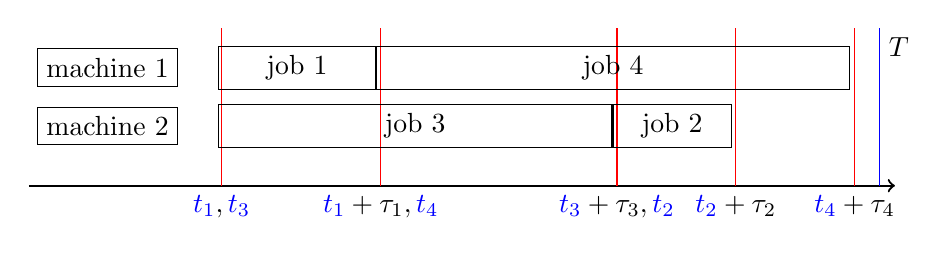
\begin{tikzpicture}
                \draw[thick,->] (-1,-1.5) -- (10,-1.5);

                \draw[color=red] (1.45,0.5) -- (1.45,-1.5);
                \draw (1.45,-1.5) -- (1.45,-1.5)
                            node[anchor=north] {$ \textcolor{blue}{t_1}, \textcolor{blue}{t_3} $};

                \draw[color=red] (3.47,0.5) -- (3.47,-1.5);
                \draw (3.47,-1.5) -- (3.47,-1.5)
                            node[anchor=north] {$ \textcolor{blue}{t_1}+\tau_1, \textcolor{blue}{t_4} $};

                \draw[color=red] (6.47,0.5) -- (6.47,-1.5);
                \draw (6.47,-1.5) -- (6.47,-1.5)
                            node[anchor=north] {$ \textcolor{blue}{t_3}+\tau_3, \textcolor{blue}{t_2} $};

                \draw[color=red] (7.98,0.5) -- (7.98,-1.5);
                \draw (7.98,-1.5) -- (7.98,-1.5)
                            node[anchor=north] {$ \textcolor{blue}{t_2}+\tau_2 $};

                \draw[color=red] (9.49,0.5) -- (9.49,-1.5);
                \draw (9.49,-1.5) -- (9.49,-1.5)
                            node[anchor=north] {$ \textcolor{blue}{t_4}+\tau_4 $};

                \draw[color=blue] (9.8,0.5) -- (9.8,-1.5);
                \draw (9.8,0.5) -- (9.8,0.5)
                            node[anchor=north west] {$ T $};

                \node [draw] (m1) at (0,0) {machine 1};
                \node [draw, below = 0.25cm of m1] (m2) {machine 2};
                \node [draw, minimum width=2cm,
                        right = 0.5cm of m1]
                                        (job1) {job 1};
                \node [draw, minimum width=6cm,
                        right = 0cm of job1]
                                        (job4) {job 4};
                \node [draw, minimum width=5cm,
                        right = 0.5cm of m2]
                                        (job3) {job 3};
                \node [draw, minimum width=1.5cm,
                        right = 0cm of job3]
                                        (job2) {job 2};
            \end{tikzpicture}
        \end{figure}
    \begin{itemize}
        \item $ \textcolor{blue}{p_{mj}} = True $
        if job $ j $ is scheduled
        on machine $ m $:
        \\
        e.g. $ \textcolor{blue}{p_{11}} = \textcolor{blue}{p_{14}} = \textcolor{blue}{p_{23}} = \textcolor{blue}{p_{22}} = True $
        \item job $ i $ starts at $ \textcolor{blue}{t_i} $
        and lasts $ \tau_i $
        \item a machine cannot process two or more jobs
        simultaneously:
        \\
        $ (\textcolor{blue}{p_{mi}} \land \textcolor{blue}{p_{mj}}) \rightarrow ((\textcolor{blue}{t_i} + \tau_i \le \textcolor{blue}{t_j}) \lor (\textcolor{blue}{t_j} + \tau_j \le \textcolor{blue}{t_i})) \quad \Leftrightarrow $
        \\
        $ (\textcolor{blue}{p_{mi}} \land \textcolor{blue}{p_{mj}}) \rightarrow ((\textcolor{blue}{t_i} - \textcolor{blue}{t_j} \le -\tau_i) \lor (\textcolor{blue}{t_j} - \textcolor{blue}{t_i} \le -\tau_j)) $
        \item the overall processing time should not exceed $ T $:
        \\
        $ \textcolor{blue}{t_i} + \tau_i \le T \quad \Leftrightarrow \quad \textcolor{blue}{t_i} - 0 \le T -\tau_i $
    \end{itemize}
    \end{frame}



    \begin{frame}
        \frametitle{Example Problem: Job Scheduling}
        \begin{equation*}
            \begin{aligned}
                \phi &= \bigwedge_{j=1}^{4} (\textcolor{blue}{p_{1j}} \lor \textcolor{blue}{p_{2j}}) \quad \land \\
            \end{aligned}
        \end{equation*}
        \begin{center}Each task is executed on at least one machine\end{center}
        \pause
        \begin{equation*}
        \begin{aligned}
        & \bigwedge_{j=1}^{4} ((\textcolor{blue}{p_{1j}} \rightarrow \neg \textcolor{blue}{p_{2j}}) \land (\textcolor{blue}{p_{2j}} \rightarrow \neg \textcolor{blue}{p_{1j}})) \quad \land \\
        \end{aligned}
        \end{equation*}
        \begin{center}Each task can be scheduled on one machine only\end{center}
        \pause
        \begin{equation*}
        \begin{aligned}
        & \bigwedge_{j=1}^{4} (\textcolor{blue}{t_j} \ge 0) \; \land \; \bigwedge_{j=1}^{4} (\textcolor{blue}{t_j} \le T-\tau_j) \quad \land \\
        \end{aligned}
        \end{equation*}
        \begin{center}General time constraints\end{center}
        \pause
        \begin{equation*}
        \begin{aligned}
        & \bigwedge_{m=1}^{2} \bigwedge_{i=1}^{3} \bigwedge_{j=i+1}^{4} ((\textcolor{blue}{p_{mi}} \land \textcolor{blue}{p_{mj}}) \rightarrow ((\textcolor{blue}{t_i}-\textcolor{blue}{t_j} \le -\tau_i) \lor (\textcolor{blue}{t_j}-\textcolor{blue}{t_i} \le -\tau_j))) \\
        \end{aligned}
        \end{equation*}
        \begin{center}No time overlap rule\end{center}
    \end{frame}



    \begin{frame}
        \frametitle{SAT Checking}
        \begin{columns}[T]
            \begin{column}{.4\textwidth}
                \begin{equation*}
                    \phi = (a \lor b) \land (b \lor c) \land (c \lor a) \land \dots
                \end{equation*}
                SAT checking = intelligent search in the model space.
                The model space can be represented as a tree.
            \end{column}
            \begin{column}{.4\textwidth}
                \begin{figure}[htb]
                    \resizebox {1.33\linewidth} {!} {
                        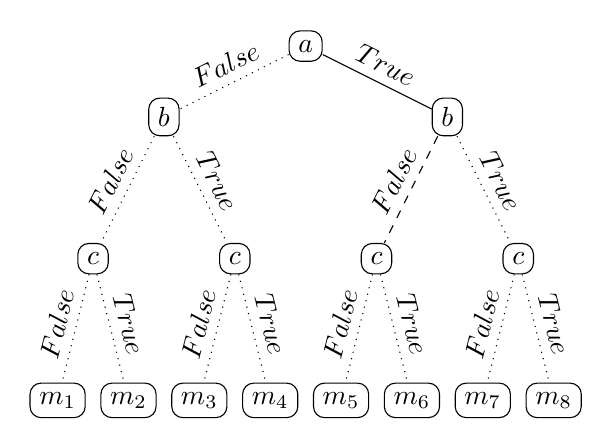
\begin{tikzpicture}[scale=0.9,state/.style={draw, rounded corners, fill=none,text centered, text=black}]
    \node[state] (n1) at (3.5, 5) {$a$};

    \node[state] (n2) at (1.5, 4) {$b$};
    \node[state] (n3) at (5.5, 4) {$b$};
    
    \node[state] (n4) at (0.5, 2) {$c$};
    \node[state] (n5) at (2.5, 2) {$c$};
    \node[state] (n6) at (4.5, 2) {$c$};
    \node[state] (n7) at (6.5, 2) {$c$};

    \node[state] (n8) at (0, 0) {$m_1$};
    \node[state] (n9) at (1, 0) {$m_2$};
    \node[state] (n10) at (2, 0) {$m_3$};
    \node[state] (n11) at (3, 0) {$m_4$};
    \node[state] (n12) at (4, 0) {$m_5$};
    \node[state] (n13) at (5, 0) {$m_6$};
    \node[state] (n14) at (6, 0) {$m_7$};
    \node[state] (n15) at (7, 0) {$m_8$};

    \path[every node/.style={sloped,anchor=south,auto=false}]
        (n1) edge[dotted] node {$False$} (n2)
        (n1) edge node {$True$} (n3)

        (n2) edge[dotted] node {$False$} (n4)
        (n2) edge[dotted] node {$True$} (n5)
        (n3) edge[dashed] node {$False$} (n6)
        (n3) edge[dotted] node {$True$} (n7)

        (n4) edge[dotted] node {$False$} (n8)
        (n4) edge[dotted] node {$True$} (n9)
        (n5) edge[dotted] node {$False$} (n10)
        (n5) edge[dotted] node {$True$} (n11)
        (n6) edge[dotted] node {$False$} (n12)
        (n6) edge[dotted] node {$True$} (n13)
        (n7) edge[dotted] node {$False$} (n14)
        (n7) edge[dotted] node {$True$} (n15);
\end{tikzpicture}

                    }
                \end{figure}
            \end{column}
        \end{columns}
    \end{frame}



    \begin{frame}
        \frametitle{SAT Checking}
        \begin{figure}[htb]
            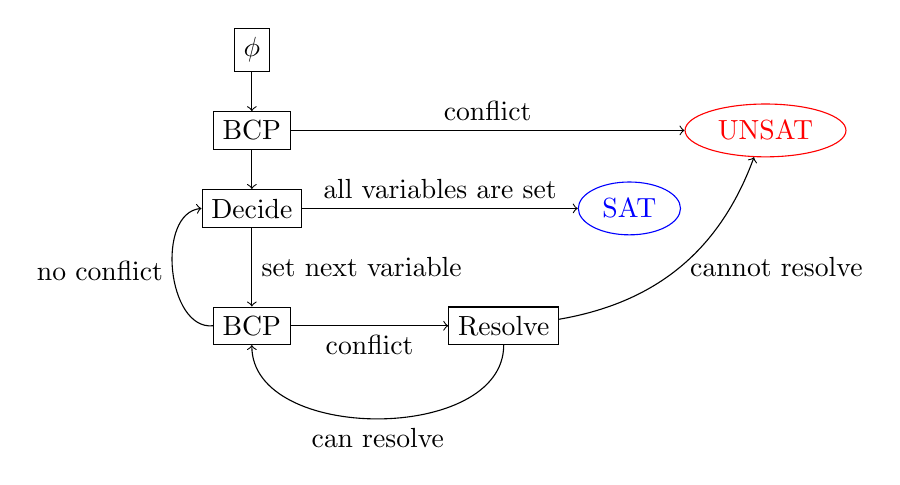
\begin{tikzpicture}
            \tikzstyle{block} = [draw, rectangle]

            \node [block] (formula) {$ \phi $};
            \node [block, below = 0.5cm of formula] (BCP) {BCP};
            \node [draw, ellipse, color=red, right = 5cm of BCP] (unsat) {UNSAT};
            \node [block, below = 0.5cm of BCP] (decide) {Decide};
            \node [draw, ellipse, color=blue, right = 3.5cm of decide] (sat) {SAT};
            \node [block, below = 1cm of decide] (BCP2) {BCP};
            \node [block, right = 2cm of BCP2] (resolve) {Resolve};
            \draw[->] (formula) -- (BCP);
            \draw [->] (BCP) -- node[anchor=south] {conflict} (unsat);
            \draw [->] (BCP) -- (decide);
            \draw [->] (decide) -- node[anchor=south] {all variables are set} (sat);
            \draw [->] (decide) -- node[anchor=west] {set next variable} (BCP2);
            \draw [->] (BCP2) -- node[anchor=north] {conflict} (resolve);
            \draw [->] (BCP2) edge[bend left=90] node[anchor=east] {no conflict} (decide);
            \draw [->] (resolve) edge[bend right=30] node[anchor=west] {cannot resolve} (unsat);
            \draw [->] (resolve) edge[bend left=90] node[anchor=north] {can resolve} (BCP2);
            \end{tikzpicture}
        \end{figure}
    \end{frame}



    \begin{frame}
        \frametitle{SAT Checking}
        \begin{figure}[htb]
            \resizebox {0.55\linewidth} {!} {
                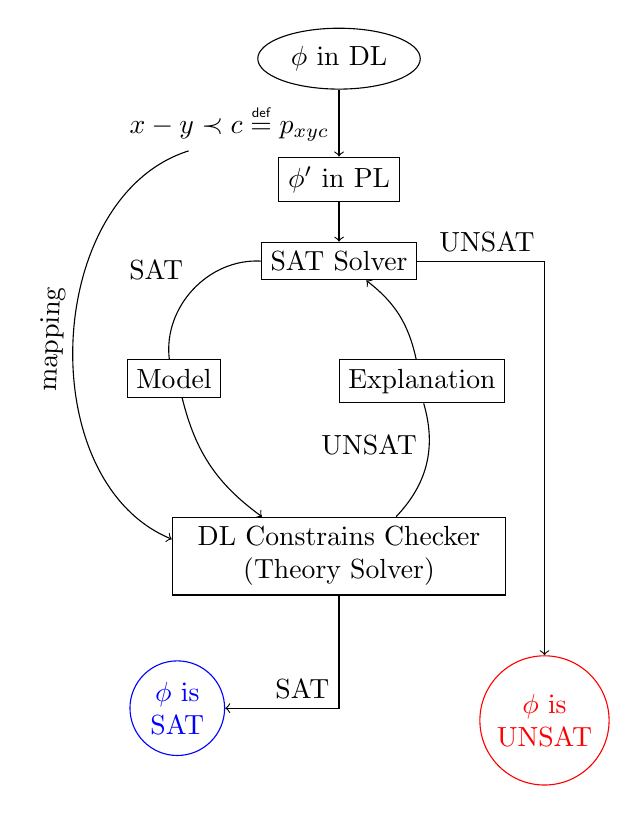
\begin{tikzpicture}
                \tikzstyle{block} = [draw, rectangle]
                
                \node [draw, ellipse] (dl) {$ \phi $ in DL};
                \node [block, below = 0.85cm of dl] (pl) {$ \phi' $ in PL};
                \node [block, below = 0.5cm of pl] (sat-solver) {SAT Solver};
                \node [block, below left = 1cm and 0.5cm of sat-solver] (model) {Model};
                \node [block, below right = 1cm and -1cm of sat-solver] (explanation) {Explanation};
                \node [block, below = 3cm of sat-solver, text width=4cm, align=center] (theory-solver) {DL Constrains Checker (Theory Solver)};
                \node [draw, circle, color=blue, inner sep=0pt, text width=1cm, align=center, below left = 1cm and -0.5cm of theory-solver] (sat) {$ \phi $ is SAT};
                \node [draw, circle, color=red, inner sep=0pt, text width=1.5cm, align=center, below right = 1cm and -0.1cm of theory-solver] (unsat) {$ \phi $ is UNSAT};
                
                \draw [->] (dl) -- node[anchor=east, name=substitution] {$ x - y \prec c \eqbydef p_{xyc} $} (pl);
                \draw [->] (pl) -- (sat-solver);
                \draw [->] (substitution) edge[bend right=70] node[anchor=south, sloped] {mapping} (theory-solver);
                \draw [-] (sat-solver.west) edge[bend right=50] node[anchor=south east] {SAT} (model);
                \draw [->] (model) edge[bend right=20] (theory-solver);
                \draw [->] (sat-solver) -| node[anchor=south east] {UNSAT} (unsat);
                \draw [-] (theory-solver) edge[bend right=30] node[anchor=south east] {UNSAT} (explanation);
                \draw [->] (explanation) edge[bend right=20] (sat-solver);
                \draw [->] (theory-solver) |- node[anchor=south east] {SAT} (sat);
                \end{tikzpicture}
            }
            \caption{Lazy approach}
        \end{figure}
    \end{frame}



    \begin{frame}
        \frametitle{SAT Checking}
        \begin{figure}[htb]
            \resizebox {0.55\linewidth} {!} {
                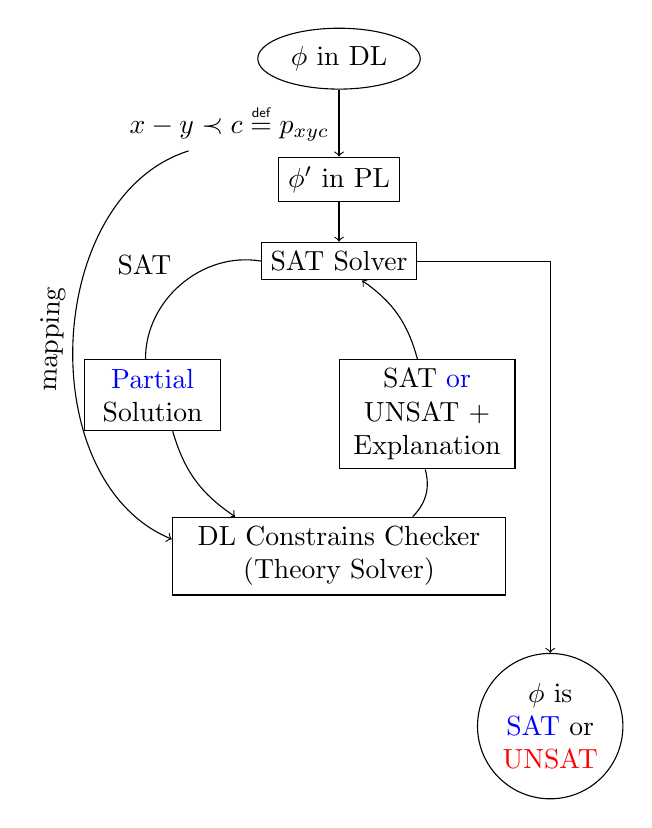
\begin{tikzpicture}
                \tikzstyle{block} = [draw, rectangle]
                
                \node [draw, ellipse] (dl) {$ \phi $ in DL};
                \node [block, below = 0.85cm of dl] (pl) {$ \phi' $ in PL};
                \node [block, below = 0.5cm of pl] (sat-solver) {SAT Solver};
                \node [block, below left = 1cm and 0.5cm of sat-solver, text width=1.5cm, align=center] (model) {\textcolor{blue}{Partial} Solution};
                \node [block, below right = 1cm and -1cm of sat-solver, text width=2cm, align=center] (explanation) {SAT \textcolor{blue}{or} UNSAT + Explanation};
                \node [block, below = 3cm of sat-solver, text width=4cm, align=center] (theory-solver) {DL Constrains Checker (Theory Solver)};
                \node [draw, circle, inner sep=0pt, text width=1.5cm, align=center, below right = 1cm and -0.1cm of theory-solver] (unsat) {$ \phi $ is \textcolor{blue}{SAT} or \textcolor{red}{UNSAT}};
                
                \draw [->] (dl) -- node[anchor=east, name=substitution] {$ x - y \prec c \eqbydef p_{xyc} $} (pl);
                \draw [->] (pl) -- (sat-solver);
                \draw [->] (substitution) edge[bend right=70] node[anchor=south, sloped] {mapping} (theory-solver);
                \draw [-] (sat-solver.west) edge[bend right=50] node[anchor=south east] {SAT} (model);
                \draw [->] (model) edge[bend right=20] (theory-solver);
                \draw [->] (sat-solver) -| (unsat);
                \draw [-] (theory-solver) edge[bend right=30] (explanation);
                \draw [->] (explanation) edge[bend right=20] (sat-solver);
                \end{tikzpicture}
            }
            \caption{Incremental approach}
        \end{figure}
    \end{frame}



    \begin{frame}
        \frametitle{Constraint Graph And Negative Cycles}
        \begin{columns}[T]
            \begin{column}{.4\textwidth}
                \begin{figure}[htb]
                    \resizebox {1.2\linewidth} {!} {
                        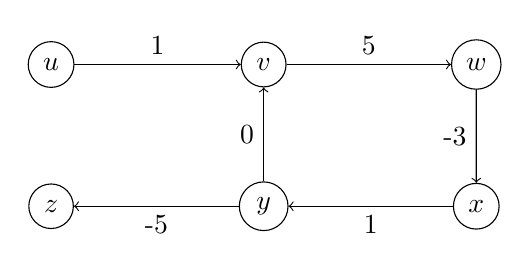
\begin{tikzpicture}[scale=0.9,state/.style={draw, circle, fill=none,text centered, text=black}]
                        \node[state] (u) at (0, 2) {$u$};
                        \node[state] (v) at (3, 2) {$v$};
                        \node[state] (w) at (6, 2) {$w$};
                        \node[state] (x) at (6, 0) {$x$};
                        \node[state] (y) at (3, 0) {$y$};
                        \node[state] (z) at (0, 0) {$z$};
                        \draw [->] (u) -- node[anchor=south] {1} (v);
                        \draw [->] (v) -- node[anchor=south] {5} (w);
                        \draw [->] (w) -- node[anchor=east] {-3} (x);
                        \draw [->] (x) -- node[anchor=north] {1} (y);
                        \draw [->] (y) -- node[anchor=north] {-5} (z);
                        \draw [->] (y) -- node[anchor=east] {0} (v);
                        \end{tikzpicture}
                        
                    }
                \end{figure}
                \begin{equation*}
                    \begin{aligned}
                    & (u-v < 1) \\
                    \land \; & (v-w < 5) \\
                    \land \; & (w-x \leq -3) \\
                    \land \; & (x-y < 1) \\
                    \land \; & (y-z \leq -5) \\
                    \land \; & (y-v \leq 0) \\
                    \end{aligned}
                \end{equation*}
                \begin{center}
                    \textcolor{blue}{SAT}
                \end{center}
            \end{column}
            \begin{column}{.4\textwidth}
                \begin{figure}[htb]
                    \resizebox {1.2\linewidth} {!} {
                        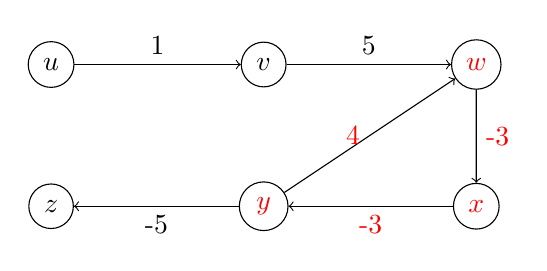
\begin{tikzpicture}[scale=0.9,state/.style={draw, circle, fill=none,text centered, text=black}]
                        \node[state] (u) at (0, 2) {$u$};
                        \node[state] (v) at (3, 2) {$v$};
                        \node[state] (w) at (6, 2) {$\textcolor{red}{w}$};
                        \node[state] (x) at (6, 0) {$\textcolor{red}{x}$};
                        \node[state] (y) at (3, 0) {$\textcolor{red}{y}$};
                        \node[state] (z) at (0, 0) {$z$};
                        \draw [->] (u) -- node[anchor=south] {1} (v);
                        \draw [->] (v) -- node[anchor=south] {5} (w);
                        \draw [->] (w) -- node[anchor=west] {\textcolor{red}{-3}} (x);
                        \draw [->] (x) -- node[anchor=north] {\textcolor{red}{-3}} (y);
                        \draw [->] (y) -- node[anchor=north] {-5} (z);
                        \draw [->] (y) -- node[anchor=east] {\textcolor{red}{4}} (w);
                        \end{tikzpicture}
                    }
                \end{figure}
                \begin{equation*}
                    \begin{aligned}
                    & (u-v < 1) \\
                    \land \; & (v-w < 5) \\
                    \land \; & (\textcolor{red}{w-x \leq -3}) \\
                    \land \; & (\textcolor{red}{x-y < -3}) \\
                    \land \; & (y-z \leq -5) \\
                    \land \; & (\textcolor{red}{y-w < 4}) \\
                    \end{aligned}
                \end{equation*}
                \begin{center}
                    \textcolor{red}{UNSAT : $ 0 < -2 $}
                \end{center}
            \end{column}
        \end{columns}
    \end{frame}



    \begin{frame}
        \frametitle{Constraint Graph And Negative Cycles}
        \begin{itemize}
            \item First idea: enumerate all cycles
            \begin{itemize}
                \item and check if they are negative \\
                \ie correspond to conflicts
                like \eg \textcolor{blue}{$ 0 < -1 $},
                \textcolor{blue}{$ 0 \le -5 $} \etc
                \item or they have zero weight and an edge with a strict inequality \\
                \ie correspond to \textcolor{blue}{$ 0 < 0 $} conflict.
            \end{itemize}
            \item \textcolor{blue}{Any problems with this approach?}
        \end{itemize}
    \end{frame}



    \begin{frame}
        \frametitle{Constraint Graph And Negative Cycles}
        \begin{figure}[htb]
            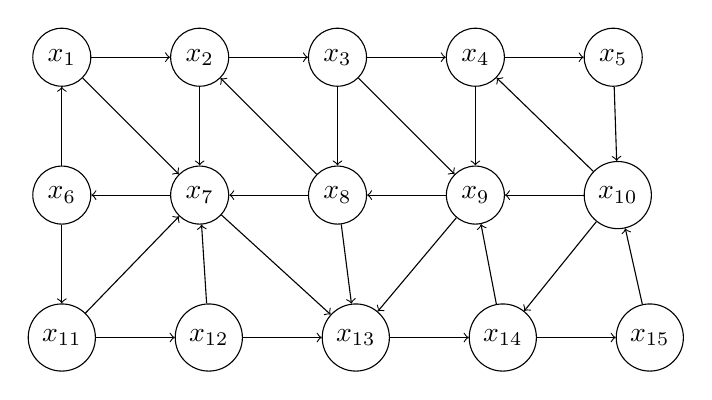
\begin{tikzpicture}
            \node [draw, circle] (x1) {$ x_1 $};
            \node [draw, circle, right = of x1] (x2) {$ x_2 $};
            \node [draw, circle, right = of x2] (x3) {$ x_3 $};
            \node [draw, circle, right = of x3] (x4) {$ x_4 $};
            \node [draw, circle, right = of x4] (x5) {$ x_5 $};
            
            \draw [->] (x1) -> (x2);
            \draw [->] (x2) -> (x3);
            \draw [->] (x3) -> (x4);
            \draw [->] (x4) -> (x5);
            
            \node [draw, circle, below = of x1] (x6) {$ x_6 $};
            \node [draw, circle, right = of x6] (x7) {$ x_7 $};
            \node [draw, circle, right = of x7] (x8) {$ x_8 $};
            \node [draw, circle, right = of x8] (x9) {$ x_9 $};
            \node [draw, circle, right = of x9] (x10) {$ x_{10} $};
            
            \draw [->] (x10) -> (x9);
            \draw [->] (x9) -> (x8);
            \draw [->] (x8) -> (x7);
            \draw [->] (x7) -> (x6);
            
            \draw [->] (x5) -> (x10);
            \draw [->] (x10) -> (x4);
            \draw [->] (x4) -> (x9);
            \draw [->] (x3) -> (x9);
            \draw [->] (x3) -> (x8);
            \draw [->] (x8) -> (x2);
            \draw [->] (x2) -> (x7);
            \draw [->] (x1) -> (x7);
            \draw [->] (x6) -> (x1);

            \node [draw, circle, below = of x6] (x11) {$ x_{11} $};
            \node [draw, circle, right = of x11] (x12) {$ x_{12} $};
            \node [draw, circle, right = of x12] (x13) {$ x_{13} $};
            \node [draw, circle, right = of x13] (x14) {$ x_{14} $};
            \node [draw, circle, right = of x14] (x15) {$ x_{15} $};
            
            \draw [->] (x11) -> (x12);
            \draw [->] (x12) -> (x13);
            \draw [->] (x13) -> (x14);
            \draw [->] (x14) -> (x15);
            
            \draw [->] (x6) -> (x11);
            \draw [->] (x11) -> (x7);
            \draw [->] (x12) -> (x7);
            \draw [->] (x7) -> (x13);
            \draw [->] (x8) -> (x13);
            \draw [->] (x9) -> (x13);
            \draw [->] (x14) -> (x9);
            \draw [->] (x10) -> (x14);
            \draw [->] (x15) -> (x10);
            \end{tikzpicture}
        \end{figure}
        \begin{itemize}
            \item \textcolor{blue}{Problem:} a graph can have
            an enormous number of cycles
            \item \Eg extreme case: \textcolor{blue}{fully connected}
            \textit{directed} graph with $ n $ vertices
            \begin{itemize}
                \item Number of \textcolor{blue}{simple} cycles =
                $ \sum_{i=2}^{n} \binom{i}{n}
                \cdot (i-1)! $
                \item Factorial grows even faster than exponent
                $ \Rightarrow $ the problem becomes intractable.
            \end{itemize}
        \end{itemize}
    \end{frame}



    \begin{frame}
        \frametitle{Constraint Graph And Negative Cycles}
        \begin{itemize}
            \item Use Bellman-Ford algorithm for this
            task~\textcolor{blue}{[Cormen \etal 2009]}
            \begin{itemize}
                \item $ O(|V| \cdot |E|) $ time complexity
                \item $ s \in V $ -- source vertex
                (can be selected \eg randomly)
                \item $ \Gamma = (V,E,weight) $ -- directed graph
                \item $ d \in V \mapsto \mathbb{R} $ -- distance estimate function
                \item Note: the algorithm runs once for the whole graph,
                not once for each vertex (\ie $ |V| $ times).
            \end{itemize}
        \end{itemize}
        \begin{algorithm}{Bellman-Ford} { \Gamma, s }
            \mathrm{set} \;\;\; d(x) = \infty \;\;\; \forall x \in V \\
            d(s) = 0
            \pause
            \\
            \begin{FOR}{i = 1 \; \mathrm{to} \; |V|-1}
                \begin{FOR}{\mathrm{each \; edge} \; (x,y) \in E}
                    \begin{IF}{\textcolor{blue}{d(x) + weight(x,y) < d(y)}}
                        \textcolor{blue}{
                            d(y) = d(x) + weight(x,y)
                        }
                    \end{IF}
                \end{FOR}
            \end{FOR}
            \pause
            \\
            \begin{FOR}{\mathrm{each \; edge} \; (x,y) \in E}
                \begin{IF}{d(x) + weight(x,y) < d(y)}
                    \RETURN False \; (
                    \textcolor{blue}{\Rightarrow \mathrm{negative\;cycle\;detected}}
                    )
                \end{IF}
            \end{FOR}
            \pause
            \\
            \RETURN True
            \; (
            \textcolor{blue}{\Rightarrow \mathrm{no\;negative\;cycles}}
            )
        \end{algorithm}
    \end{frame}



    \begin{frame}
        \frametitle{Constraint Graph And Negative Cycles}
        \begin{itemize}
            \item \textcolor{blue}{[Cotton \etal 2004]}
            uses the \textcolor{blue}{admissible graph}
            $ \Gamma_d $ to find
            a negative or zero weight cycle in the original
            constraint graph~$ \Gamma $
            \item Terminology:
            \begin{itemize}
                \item Reduced cost function
                $ r(x,y) = weight(x,y) + d(x) - d(y) $
                \item Admissible edge:
                $ r(x,y) \; \textcolor{blue}{\leq} \; 0 $
                \item Admissible graph $ \Gamma_d $ -- a graph
                consisting of admissible edges
            \end{itemize}
            \item Implications:
            \begin{itemize}
                \item $ \Gamma_d $ is \textcolor{blue}{dynamic}
                because it depends
                on $ d $ which
                \textcolor{blue}{changes during
                the execution of the algorithm}
                \item If $ r(x,y) < 0 $ then the edge $ (x,y) $
                can be "relaxed" \ie used to improve $ d(y) $
                \item $ \Gamma_d $ consists of
                edges which might potentially be used to improve $ d $
                \item Intuition: if $ \Gamma_d $ has a
                \textcolor{blue}{cycle} then
                this cycle might be used to
                \textcolor{blue}{update $ d $ infinitely}
            \end{itemize}
        \end{itemize}
    \end{frame}



    \begin{frame}
    \frametitle{Constraint Graph And Negative Cycles}
    \begin{theorem}
        \label{the:neg-cycle-in-cg}
        Given a constraint graph $ \Gamma $ \\
        and \\
        a \textcolor{blue}{series} of distance estimating \\
        functions $ (d_0, d_1, d_2, d_3, \dots) $, \\
        $ \Gamma $ has a negative or zero cycle \\
        if and only if \\
        \textcolor{blue}{
            $ \Gamma_d $ has a cycle under some
            distance estimate $ d_k $.
        }
        \begin{proof}
            see~\textcolor{blue}{[Cotton~\etal~2004]}.
        \end{proof}
    \end{theorem}
    \begin{center}
        Note: the series $ (d_0, d_1, d_2, d_3, \dots) $ \\
        correspond to the updates of $ d $ during the run of Bellman-Ford \\
        where $ d_0(s) = 0 $ and
        $ d_0(x)=\infty \; \forall x \in V \; s.t. \; x \ne s $ \\
        are the initial distance estimates.
    \end{center}
    \end{frame}



    \begin{frame}
        \frametitle{Constraint Graph And Negative Cycles}
        \begin{columns}[T]
            \begin{column}{.48\textwidth}
                \begin{figure}[htb]
                    \resizebox {\linewidth} {!} {
                        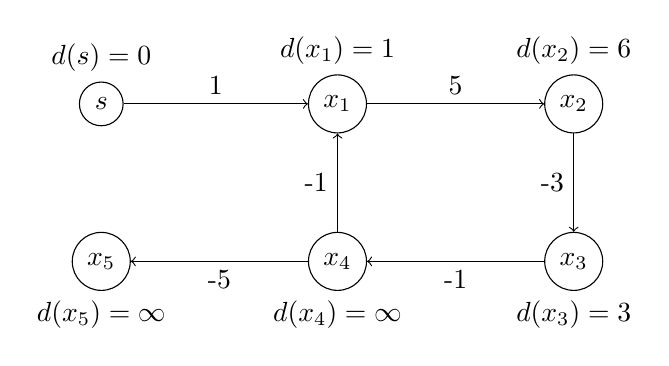
\begin{tikzpicture}[state/.style={draw, circle, fill=none,text centered, text=black}]
                        \node[state, label={$ d(s) = 0 $}] (s) at (0, 2) {$s$};
                        \node[state, label={$ d(x_1) = 1 $}] (x1) at (3, 2) {$x_1$};
                        \node[state, label={$ d(x_2) = 6 $}] (x2) at (6, 2) {$x_2$};
                        \node[state, label={-90:$ d(x_3) = 3 $}] (x3) at (6, 0) {$x_3$};
                        \node[state, label={-90:$ d(x_4) = \infty $}] (x4) at (3, 0) {$x_4$};
                        \node[state, label={-90:$ d(x_5) = \infty $}] (x5) at (0, 0) {$x_5$};
                        \draw [->] (s) -- node[anchor=south] {1} (x1);
                        \draw [->] (x1) -- node[anchor=south] {5} (x2);
                        \draw [->] (x2) -- node[anchor=east] {-3} (x3);
                        \draw [->] (x3) -- node[anchor=north] {-1} (x4);
                        \draw [->] (x4) -- node[anchor=north] {-5} (x5);
                        \draw [->] (x4) -- node[anchor=east] {-1} (x1);
                        \end{tikzpicture}
                    }
                \caption{$ \Gamma $}
                \end{figure}
            \end{column}
            \hfill
            \begin{column}{.48\textwidth}
                \begin{figure}[htb]
                    \resizebox {\linewidth} {!} {
                        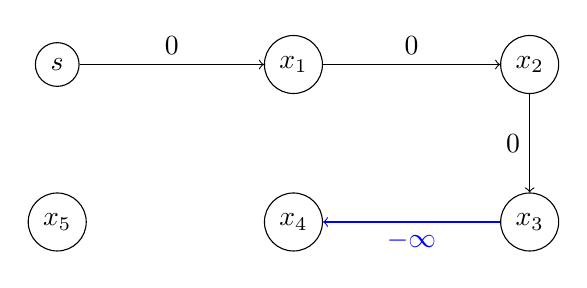
\begin{tikzpicture}[state/.style={draw, circle, fill=none, text centered, text=black}]
                        \node[state] (s) at (0, 2) {$s$};
                        \node[state] (x1) at (3, 2) {$x_1$};
                        \node[state] (x2) at (6, 2) {$x_2$};
                        \node[state] (x3) at (6, 0) {$x_3$};
                        \node[state] (x4) at (3, 0) {$x_4$};
                        \node[state] (x5) at (0, 0) {$x_5$};
                        \draw [->] (s) -- node[anchor=south] {0} (x1);
                        \draw [->] (x1) -- node[anchor=south] {0} (x2);
                        \draw [->] (x2) -- node[anchor=east] {0} (x3);
                        \draw [->, color=blue] (x3) -- node[anchor=north] {$ -\infty $} (x4);
                        \end{tikzpicture}
                    }
                    \caption{$ \Gamma_d $}
                \end{figure}
            \end{column}
        \end{columns}
        \begin{equation*}
                r(x,y) = weight(x,y) + d(x) - d(y)
        \end{equation*}
        \begin{center}
            \begin{tabular}{c c c}
                $ r(s,x_1) = 0 $ & $ r(x_1,x_2) = 0 $ & $ r(x_2,x_3) = 0 $ \\
                $ r(x_3,x_4) = -\infty $ & $ r(x_4,x_1) = \infty $ & $ r(x_4,x_5) = \varnothing $ \\
            \end{tabular}
        \end{center}
        $ \Gamma_d $ has no cycles. Let us relax the edge
        \textcolor{blue}{$ (x_3, x_4) $}
    \end{frame}




    \begin{frame}
        \frametitle{Constraint Graph And Negative Cycles}
        \begin{columns}[T]
            \begin{column}{.48\textwidth}
                \begin{figure}[htb]
                    \resizebox {\linewidth} {!} {
                        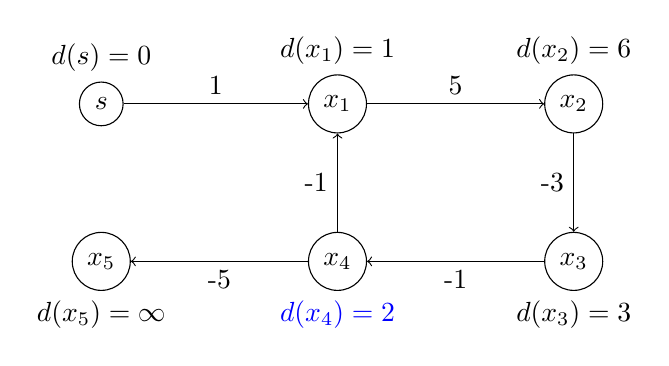
\begin{tikzpicture}[state/.style={draw, circle, fill=none,text centered, text=black}]
                        \node[state, label={$ d(s) = 0 $}] (s) at (0, 2) {$s$};
                        \node[state, label={$ d(x_1) = 1 $}] (x1) at (3, 2) {$x_1$};
                        \node[state, label={$ d(x_2) = 6 $}] (x2) at (6, 2) {$x_2$};
                        \node[state, label={-90:$ d(x_3) = 3 $}] (x3) at (6, 0) {$x_3$};
                        \node[state, label={-90:$ \textcolor{blue}{d(x_4) = 2} $}] (x4) at (3, 0) {$x_4$};
                        \node[state, label={-90:$ d(x_5) = \infty $}] (x5) at (0, 0) {$x_5$};
                        \draw [->] (s) -- node[anchor=south] {1} (x1);
                        \draw [->] (x1) -- node[anchor=south] {5} (x2);
                        \draw [->] (x2) -- node[anchor=east] {-3} (x3);
                        \draw [->] (x3) -- node[anchor=north] {-1} (x4);
                        \draw [->] (x4) -- node[anchor=north] {-5} (x5);
                        \draw [->] (x4) -- node[anchor=east] {-1} (x1);
                        \end{tikzpicture}
                    }
                    \caption{$ \Gamma $}
                \end{figure}
            \end{column}
            \hfill
            \begin{column}{.48\textwidth}
                \begin{figure}[htb]
                    \resizebox {\linewidth} {!} {
                        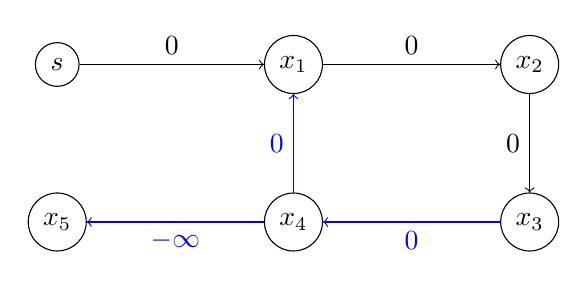
\begin{tikzpicture}[state/.style={draw, circle, fill=none, text centered, text=black}]
                        \node[state] (s) at (0, 2) {$s$};
                        \node[state] (x1) at (3, 2) {$x_1$};
                        \node[state] (x2) at (6, 2) {$x_2$};
                        \node[state] (x3) at (6, 0) {$x_3$};
                        \node[state] (x4) at (3, 0) {$x_4$};
                        \node[state] (x5) at (0, 0) {$x_5$};
                        \draw [->] (s) -- node[anchor=south] {0} (x1);
                        \draw [->] (x1) -- node[anchor=south] {0} (x2);
                        \draw [->] (x2) -- node[anchor=east] {0} (x3);
                        \draw [->, color=blue] (x3) -- node[anchor=north] {$ \textcolor{blue}{0} $} (x4);
                        \draw [->, color=blue] (x4) -- node[anchor=north] {$ \textcolor{blue}{-\infty} $} (x5);
                        \draw [->, color=blue] (x4) -- node[anchor=east] {\textcolor{blue}{0}} (x1);
                        \end{tikzpicture}
                    }
                    \caption{$ \Gamma_d $}
                \end{figure}
            \end{column}
        \end{columns}
        \begin{equation*}
            r(x,y) = weight(x,y) + d(x) - d(y)
        \end{equation*}
        \begin{center}
            \begin{tabular}{c c c}
                $ r(s,x_1) = 0 $ & $ r(x_1,x_2) = 0 $ & $ r(x_2,x_3) = 0 $ \\
                $ \textcolor{blue}{r(x_3,x_4) = 0} $ & $ \textcolor{blue}{r(x_4,x_1) = 0} $ & $ \textcolor{blue}{r(x_4,x_5) = -\infty} $ \\
            \end{tabular}
        \end{center}
        Now $ \Gamma_d $ has a cycle:
        \textcolor{blue}{$ x_1 \rightarrow x_2 \rightarrow x_3 \rightarrow x_4 \rightarrow x_1 $}.
        This cycle in $ \Gamma $ has indeed zero weight.
    \end{frame}



    \begin{frame}
        \frametitle{Constraint Graph And Negative Cycles}
        \begin{figure}[htb]
            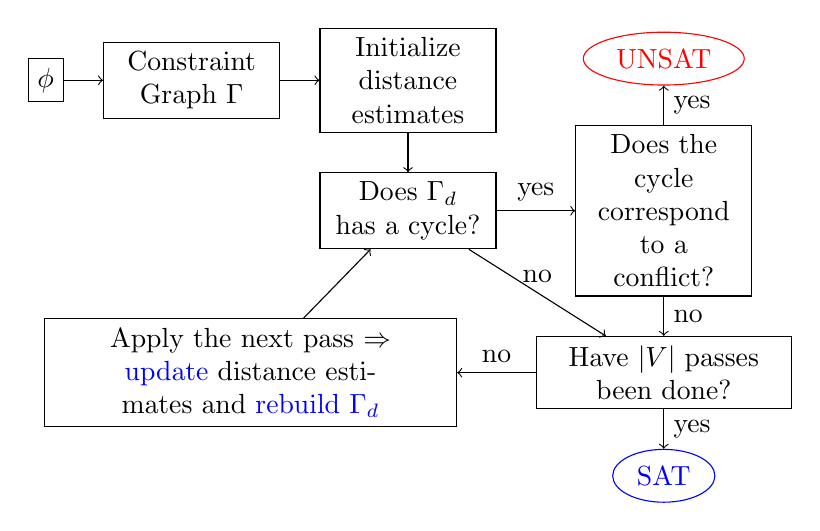
\begin{tikzpicture}
            \tikzstyle{block} = [draw, rectangle]
            \node [block] (formula) {$ \phi $};
            \node [block, right = 0.5cm of formula, text width=2cm, align=center] (cg) {Constraint Graph $ \Gamma $};
            \node [block, right = 0.5cm of cg, text width=2cm, align=center] (init1) {Initialize distance estimates};
            \node [block, below = 0.5cm of init1, text width=2cm, align=center] (checkCycle) {Does $ \Gamma_d $ has a cycle?};
            \node [block, right = of checkCycle, text width=2cm, align=center] (hasCycle) {Does the cycle correspond to a conflict?};
            \node [draw, ellipse, color=red, above = 0.5cm of hasCycle] (unsat) {UNSAT};
            \node [block, below = 0.5cm of hasCycle, text width=3cm, align=center] (admissibleEdges) {Have $ |V| $ passes been done?};
            \node [draw, ellipse, color=blue, below = 0.5cm of admissibleEdges] (sat) {SAT};
            \node [block, left = 1cm of admissibleEdges, text width=5cm, align=center] (applyGR) {Apply the next pass $ \Rightarrow $ \textcolor{blue}{update} distance estimates and \textcolor{blue}{rebuild $ \Gamma_d $}};

            \draw[->] (formula) -- (cg);
            \draw[->] (cg) -- (init1);
            \draw[->] (init1) -- (checkCycle);
            \draw[->] (checkCycle) -- node[anchor=south] {yes} (hasCycle);
            \draw[->] (checkCycle) -- node[anchor=south] {no} (admissibleEdges);
            \draw[->] (hasCycle) -- node[anchor=west] {yes} (unsat);
            \draw[->] (hasCycle) -- node[anchor=west] {no} (admissibleEdges);
            \draw [->] (admissibleEdges) -- node[anchor=west] {yes} (sat);
            \draw [->] (admissibleEdges) -- node[anchor=south] {no} (applyGR);
            \draw [->] (applyGR) -- (checkCycle);
            \end{tikzpicture}
        \end{figure}
    \end{frame}



    \begin{frame}
        \frametitle{Conclusion}
        \begin{itemize}
            \item Many timing problems (logistics, planning, scheduling,
            circuits checking) can be expressed in DL.
            Therefore it is important to have an efficient algorithm
            for checking SAT of a DL formula.
            \item Conjunction of DL constraints can be represented
            by a constraint graph $ \Gamma $.
            \begin{itemize}
                \item A negative cycle corresponds to a conflict
                $ 0 \prec c $ \\
                where \textcolor{blue}{$ c < 0 $}
                and $ \prec \in \{ <, \le \} $
                \eg \textcolor{blue}{$ 0 < -3 $},
                \textcolor{blue}{$ 0 \le -1 $} \etc
                \item A zero weight cycle with a
                \textcolor{blue}{strict inequality}
                edge corresponds to a conflict
                \textcolor{blue}{$ 0 < 0 $}.
            \end{itemize}
            \item There is no need to enumerate all cycles in $ \Gamma $. \\
            Bellman-Ford algorithm can be used to detect a negative
            cycle in~\textcolor{blue}{$ O(|V| \cdot |E|) $} operations.
            \item A cycle in admissible graph $ \Gamma_d $
            corresponds to a negative or zero weight cycle in
            the corresponding constraint graph $ \Gamma $.
        \end{itemize}
    \end{frame}



    \begin{frame}
        \frametitle{Thank you}
        \Huge Thank you for your attention
    \end{frame}



    \begin{frame}
        \frametitle{Backup Slide. Number of simple cycles formula explained}
        \begin{columns}[T]
            \begin{column}{.4\textwidth}
                \begin{figure}[htb]
                    \resizebox {1.33\linewidth} {!} {
                        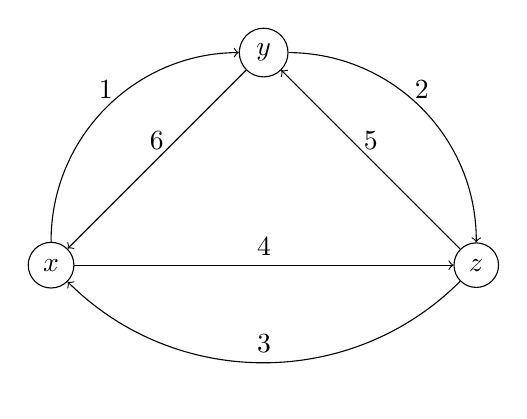
\begin{tikzpicture}[scale=0.9,state/.style={draw, circle, fill=none,text centered, text=black}]
                        \node[state] (x) at (0, 0) {$x$};
                        \node[state] (y) at (3, 3) {$y$};
                        \node[state] (z) at (6, 0) {$z$};
                        \draw [->] (x) edge[bend left=45] node[anchor=south] {$ 1 $} (y);
                        \draw [->] (y) edge[bend left=45] node[anchor=south] {$ 2 $} (z);
                        \draw [->] (z) edge[bend left=45] node[anchor=south] {$ 3 $} (x);
                        \draw [->] (x) -- node[anchor=south] {$ 4 $} (z);
                        \draw [->] (z) -- node[anchor=south] {$ 5 $} (y);
                        \draw [->] (y) -- node[anchor=south] {$ 6 $} (x);
                        \end{tikzpicture}
                    }
                \end{figure}
                \begin{itemize}
                    \item a fully connected
                    \textit{directed} graph
                    with $ n $ vertices.
                    \item Number of \textit{simple} cycles =
                    $ \sum_{i=2}^{n} \binom{i}{n}
                    \cdot (i-1)! $
                \end{itemize}
            \end{column}
            \begin{column}{.4\textwidth}
            \begin{itemize}
                \item Example for \textcolor{blue}{$ i = 3 $}
                (Figure on the left)
                \item There are $ i! = 6 $
                permutations of the vertices which
                describe 2 cycles:
                \begin{equation*}
                \begin{aligned}
                (x,y,z), (y,z,x), (z,x,y) \\
                (x,z,y), (z,y,x), (y,x,z) \\
                \end{aligned}
                \end{equation*}
                \item Each cycle is described by $ i $
                permutations which can be produced
                from each other by \textcolor{blue}{shifting}.
                Therefore, there are
                $ \frac{i!}{i} = (i-1)! $ cycles.
            \end{itemize}
            \end{column}
        \end{columns}
    \end{frame}



    \begin{frame}
    \frametitle{Backup Slide. Multiple runs of Bellman-Ford}
    \begin{figure}[htb]
        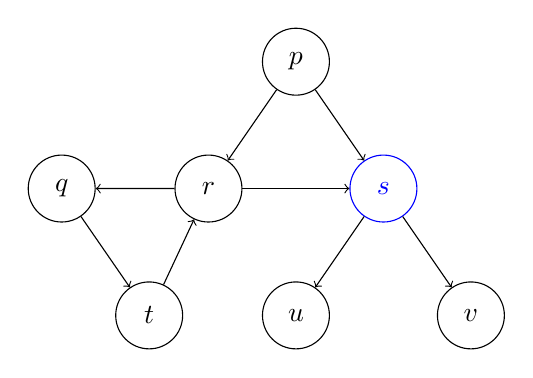
\begin{tikzpicture}[scale=0.9,state/.style={draw, circle, fill=none,text centered, text=black}]
        \tikzstyle{vertex} = [draw, circle, minimum size=0.85cm]
        \node[vertex] (p) {$p$};
        \node[vertex, below left = 1cm and 0.5cm of p] (r) {$r$};
        \node[vertex, left = 1cm of r] (q) {$q$};
        \node[vertex, below right = 1cm and 0.5cm of p, color=blue] (s) {$s$};
        \node[vertex, below right = 1cm and 0.5cm of q] (t) {$t$};
        \node[vertex, below left = 1cm and 0.5cm of s] (u) {$u$};
        \node[vertex, below right = 1cm and 0.5cm of s] (v) {$v$};

        \draw [->] (p) -- (r);
        \draw [->] (p) -- (s);
        \draw [->] (r) -- (q);
        \draw [->] (q) -- (t);
        \draw [->] (t) -- (r);
        \draw [->] (s) -- (u);
        \draw [->] (s) -- (v);
        \draw [->] (r) -- (s);
        \end{tikzpicture}
    \end{figure}
    \vfill
    \begin{center}
        In this example each edge has weight \textcolor{blue}{-1}. \\
        Suppose that \textcolor{blue}{$ s $}
        is selected as the source vertex.
    \end{center}
    \end{frame}



    \begin{frame}
    \frametitle{Backup Slide. Multiple runs of Bellman-Ford}
    \begin{figure}[htb]
        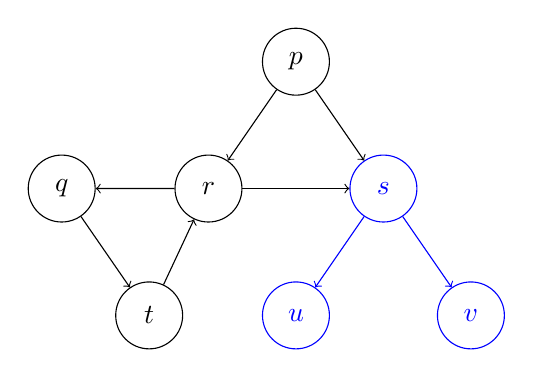
\begin{tikzpicture}[scale=0.9,state/.style={draw, circle, fill=none,text centered, text=black}]
        \tikzstyle{vertex} = [draw, circle, minimum size=0.85cm]
        \node[vertex] (p) {$p$};
        \node[vertex, below left = 1cm and 0.5cm of p] (r) {$r$};
        \node[vertex, left = 1cm of r] (q) {$q$};
        \node[vertex, below right = 1cm and 0.5cm of p, color=blue] (s) {$s$};
        \node[vertex, below right = 1cm and 0.5cm of q] (t) {$t$};
        \node[vertex, below left = 1cm and 0.5cm of s, color=blue] (u) {$u$};
        \node[vertex, below right = 1cm and 0.5cm of s, color=blue] (v) {$v$};
        
        \draw [->] (p) -- (r);
        \draw [->] (p) -- (s);
        \draw [->] (r) -- (q);
        \draw [->] (q) -- (t);
        \draw [->] (t) -- (r);
        \draw [->, color=blue] (s) -- (u);
        \draw [->, color=blue] (s) -- (v);
        \draw [->] (r) -- (s);
        \end{tikzpicture}
    \end{figure}
    \vfill
    \begin{center}
        Bellman-Ford processes only a subgraph. \\
        No cycles have been detected.
    \end{center}
    \end{frame}



    \begin{frame}
    \frametitle{Backup Slide. Multiple runs of Bellman-Ford}
    \begin{figure}[htb]
        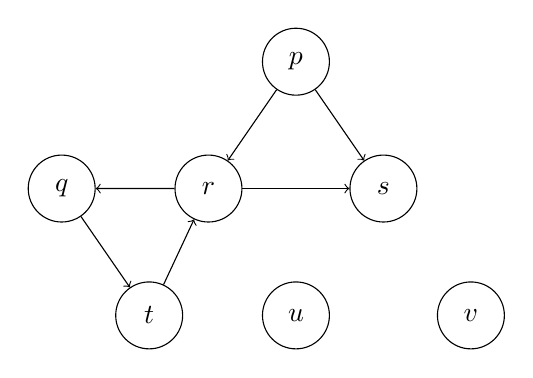
\begin{tikzpicture}[scale=0.9,state/.style={draw, circle, fill=none,text centered, text=black}]
        \tikzstyle{vertex} = [draw, circle, minimum size=0.85cm]
        \node[vertex] (p) {$p$};
        \node[vertex, below left = 1cm and 0.5cm of p] (r) {$r$};
        \node[vertex, left = 1cm of r] (q) {$q$};
        \node[vertex, below right = 1cm and 0.5cm of p] (s) {$s$};
        \node[vertex, below right = 1cm and 0.5cm of q] (t) {$t$};
        \node[vertex, below left = 1cm and 0.5cm of s] (u) {$u$};
        \node[vertex, below right = 1cm and 0.5cm of s] (v) {$v$};
        
        \draw [->] (p) -- (r);
        \draw [->] (p) -- (s);
        \draw [->] (r) -- (q);
        \draw [->] (q) -- (t);
        \draw [->] (t) -- (r);
        \draw [->] (r) -- (s);
        \end{tikzpicture}
    \end{figure}
    \vfill
    \begin{center}
        Discard the edges that have been processed \\
        because \textcolor{blue}{we do not need to process them twice}. \\
        Select the next source vertex and run Bellman-Ford again.
    \end{center}
    \end{frame}



    \begin{frame}
    \frametitle{Backup Slide. Multiple runs of Bellman-Ford}
    \begin{figure}[htb]
        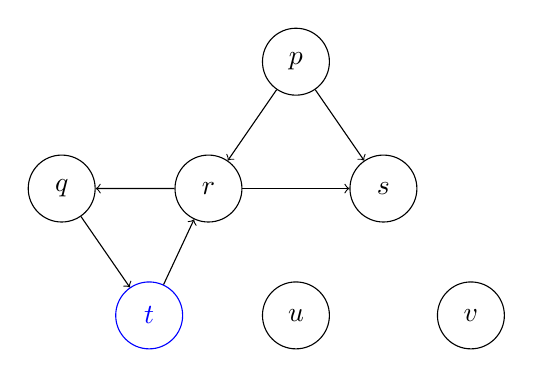
\begin{tikzpicture}[scale=0.9,state/.style={draw, circle, fill=none,text centered, text=black}]
        \tikzstyle{vertex} = [draw, circle, minimum size=0.85cm]
        \node[vertex] (p) {$p$};
        \node[vertex, below left = 1cm and 0.5cm of p] (r) {$r$};
        \node[vertex, left = 1cm of r] (q) {$q$};
        \node[vertex, below right = 1cm and 0.5cm of p] (s) {$s$};
        \node[vertex, below right = 1cm and 0.5cm of q, color=blue] (t) {$t$};
        \node[vertex, below left = 1cm and 0.5cm of s] (u) {$u$};
        \node[vertex, below right = 1cm and 0.5cm of s] (v) {$v$};
        
        \draw [->] (p) -- (r);
        \draw [->] (p) -- (s);
        \draw [->] (r) -- (q);
        \draw [->] (q) -- (t);
        \draw [->] (t) -- (r);
        \draw [->] (r) -- (s);
        \end{tikzpicture}
    \end{figure}
    \vfill
    \begin{center}
        Suppose, the next source vertex is \textcolor{blue}{$ t $}.
    \end{center}
    \end{frame}



    \begin{frame}
    \frametitle{Backup Slide. Multiple runs of Bellman-Ford}
    \begin{figure}[htb]
        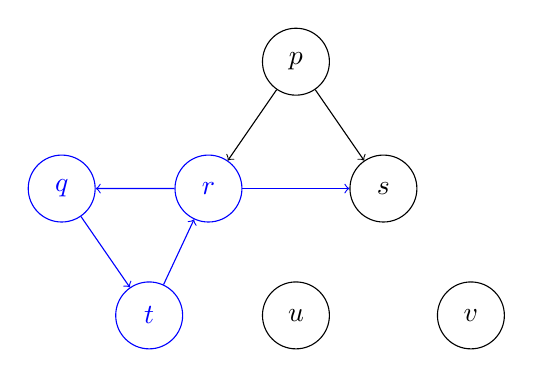
\begin{tikzpicture}[scale=0.9,state/.style={draw, circle, fill=none,text centered, text=black}]
        \tikzstyle{vertex} = [draw, circle, minimum size=0.85cm]
        \node[vertex] (p) {$p$};
        \node[vertex, below left = 1cm and 0.5cm of p, color=blue] (r) {$r$};
        \node[vertex, left = 1cm of r, color=blue] (q) {$q$};
        \node[vertex, below right = 1cm and 0.5cm of p] (s) {$s$};
        \node[vertex, below right = 1cm and 0.5cm of q, color=blue] (t) {$t$};
        \node[vertex, below left = 1cm and 0.5cm of s] (u) {$u$};
        \node[vertex, below right = 1cm and 0.5cm of s] (v) {$v$};
        
        \draw [->] (p) -- (r);
        \draw [->] (p) -- (s);
        \draw [->, color=blue] (r) -- (q);
        \draw [->, color=blue] (q) -- (t);
        \draw [->, color=blue] (t) -- (r);
        \draw [->, color=blue] (r) -- (s);
        \end{tikzpicture}
    \end{figure}
    \vfill
    \begin{center}
        Bellman-Ford finds the negative cycle
        \textcolor{blue}{$ t \rightarrow r \rightarrow q \rightarrow t $}. \\
        Since \textcolor{blue}{the processed edges have been discarded}, \\
        we do not process the edges
        \textcolor{blue}{$ (s;u) $} and \textcolor{blue}{$ (s;v) $}
        again, \\
        and therefore the complexity for the whole graph stays \\
        \textcolor{blue}{$ O(|V| \cdot |E|) $} \\
        \ie multiple runs of Bellman-Ford
        \textcolor{blue}{do not increase it}.
    \end{center}
    \end{frame}
\end{document}